\documentclass[a4paper,titlepage]{article}
\usepackage[]{mcode}
\usepackage{natbib}
\usepackage[english]{babel}
\usepackage{graphicx}
\usepackage{hyperref}
\usepackage{amsthm}
\usepackage{amsmath}
\usepackage[margin=2cm]{geometry}

\begin{document}

\begin{titlepage}
	\newcommand{\HRule}{\rule{\linewidth}{0.5mm}}
	\center

	%------------------------------------------------
	%	Logo
	%------------------------------------------------

	
\includegraphics[width=0.2\textwidth]{Crest.jpg}\\[1cm]

	%------------------------------------------------
	%	Headings
	%------------------------------------------------

	\textsc{\LARGE University of Exeter}\\[1.5cm]

	\textsc{\Large College of Engineering, Mathematics and Physical Sciences}\\[0.5cm]

	\textsc{\large ECM3735 - Group 8}\\[0.5cm]

	%------------------------------------------------
	%	Title
	%------------------------------------------------

	\HRule\\[0.4cm]

	{\huge\bfseries Finding the optimal strategy for the dice game `Pig'}\\[0.4cm]

	\HRule\\[1.5cm]

	%------------------------------------------------
	%	Authors
	%------------------------------------------------

	\LARGE\textit{Authors}\\
	\begin{minipage}{0.4\textwidth}
		\begin{flushleft}
			\large
			 \textsc{650022099}\\
			 \textsc{650011537}\\
			E. \textsc{Morison}\\
			J. \textsc{Peet}\\
			L. \textsc{Sutton}
		\end{flushleft}
	\end{minipage}
	~
	\begin{minipage}{0.4\textwidth}
		\begin{flushright}
			\large
		      \textsc{650000725}\\
			 \textsc{Jones}\\
			   \textsc{650009496}\\
			 \textsc{Smith}
			\vspace*{10pt§}
		\end{flushright}
	\end{minipage}

	\vfill\vfill
	\textit{Supervisor}\\
	Dr. B. \textsc{Cooper}

	%------------------------------------------------
	%	Date
	%------------------------------------------------

	\vfill\vfill\vfill

	{\large\today}
	\vfill

	%------------------------------------------------
	%	Abstract
	%------------------------------------------------

	\newpage
	\begin{abstract}
 This is an abstract.
	\end{abstract}
\end{titlepage}

	%------------------------------------------------
	%	Contents
	%------------------------------------------------

\tableofcontents
\listoffigures
\newpage

\section{Introduction}

\subsection{Aims and objectives}
The ultimate aim of this project was to find an optimal strategy (or optimal strategies) for the dice game Pig. The optimal strategy is defined as a strategy that has the highest probability of winning when played against all other strategies. Another aim of the project was to compare our findings to the optimal strategy that T. Neller described in his 2004 paper\cite{neller2004optimal}. Finally, we looked at the psychological aspect of playing Pig; including whether human players play according to their risk preferences (risk-neutral, risk-loving or risk-averse) and whether an individual's strategy is influenced by how well his opponent is playing.\\ \\We tried to achieve these aims by pursuing the following objectives:

\begin{enumerate}
\item Use MATLAB to write a function that calculates the probability of a given strategy winning against another, thus telling us which strategy is better.

\item Develop a script that finds the best strategy to play against any given strategy, which can be used iteratively to find the final optimal strategy.

\item Combine our probability calculator and strategy optimiser to run many tests on different strategies, producing a variety of results to study.

\item Have a sample of people play Pig and record their results so we can determine whether their strategies are influenced by how well (or badly) their opponent is doing, and whether they stick to their stated risk preferences (risk-averse, risk-neutral, risk-loving).
\end{enumerate}

\subsection{A brief history of Pig}
\subsubsection{Basics of Pig}
The dice game Pig has many variations, so we chose to focus on the two-player single-die variant. When it is a player's turn, they can repeatedly roll the die as many times as they wish. The number on each roll signifies the points gained on that roll, which is added to a running total of points for the turn. These points can be banked to bring a player's turn to an end. However, all of the points in this running total are lost if the player rolls a $1$ before banking, immediately bringing their turn to an end. The aim of the game is to be the first player to have a banked total of at least $100$ points.
\\
\\
Many different strategies can be used in Pig. For example, a simple strategy would be to roll until passing a turn score of 20, then banking. A strategy can be thought of as the choice to either roll the dice, or bank the turn score, at any game state.
\\
\\
A game state is defined by the current position of the game, player P's banked score, player Q's banked score and player P's turn score. These three scores vary between zero and 100. The mistake would be to assume that this means there are $100\times100\times100 = 1$ Million game states. The reason this is not true is because many are not possible. Take a banked score of $90$ and a turn score of $50$ for example, this game would have ended a long time ago when the player reached a turn score of $10$ winning them the game! This could be called an impossible game state, because it is not possible to reach this state, playing by the rules of the game. Another type of impossible game state is with a turn score of $1$. The smallest turnscore larger than $0$ that a player can have is by rolling a $2$, giving them a turn score of $2$.
\\
\\
Let us now define a strategy as an array of choices, 1s for rolling, and 0s for banking, where the array is 3 dimensional, and containing every possible game state. Does this let us define every possible strategy or are there more variables to consider? If this does define every strategy, the next big question, and the main focus of this paper, is what is the best strategy to play? What strategy is most likely to win against any other, and be crowned the Optimal Strategy for the dice game pig.
\\
\\
At any gamestate it is possible to produce linear equations to determine if it is better to roll or bank by looking at the probability of winning from that gamestate. Suppose there are two strategies A and B. Consider that it is P's turn and they are in position ($i,j,k$) where $i$ is P's banked points, $j$ is Q's banked points, and $k$ is B's sum total of points so far on this turn. Let $P_{ijk}$ denote the probability of P winning from the current position and $Q_{jik}$ denote probability of Q winning from the equivalent position (Note that the position of $j$ and $i$ have swapped because it is from the perspective of each player). Then,
\begin{equation}\label{1.2.1.a}
P_{ijk} = \dfrac{1}{6} (1-Q_{ij0}) + \dfrac{1}{6}\sum^{6}_{r=2}P_{ijk+r}
\end{equation}
if P rolls and
\begin{equation}\label{1.2.1.b}
P_{ijk} = 1-Q_{jik}
\end{equation}
if P banks their points.
\subsubsection{Neller's work}
In \textit{Dice Games Properly Explained}, R. Knizia takes the view of each roll of the die in Pig as a bet of not rolling a $1$. He said of the best strategy, ``Whenever your accumulated points are less than 20, you should continue throwing, because the odds are in your favour.''\cite{knizia2010dice}. The issue with this claim is, as T. Neller stated, ``\textit{risking points is not the same as risking the probability of winning.}''\cite{neller2004optimal} From this, T. Neller attempted to find a more optimal solution for Pig by maximising equations \ref{1.2.1.a} and \ref{1.2.1.b}. However this was not possible as he ended up with an equation of the form $x=$max$ (A_1 x+b_1,A_2 x+b_2)$ for which there is no known general method. As a result, T. Neller implemented value iteration to calculate an accurate estimate for the probabilities at each position $(i,j,k)$ for both bank and roll. Figure \ref{figure1} shows a visual interpretation of the resulting optimal strategy. Figure 1 shows that you should roll if the current game-state is within the surface of the graph, and bank otherwise.

\begin{figure}
\centering
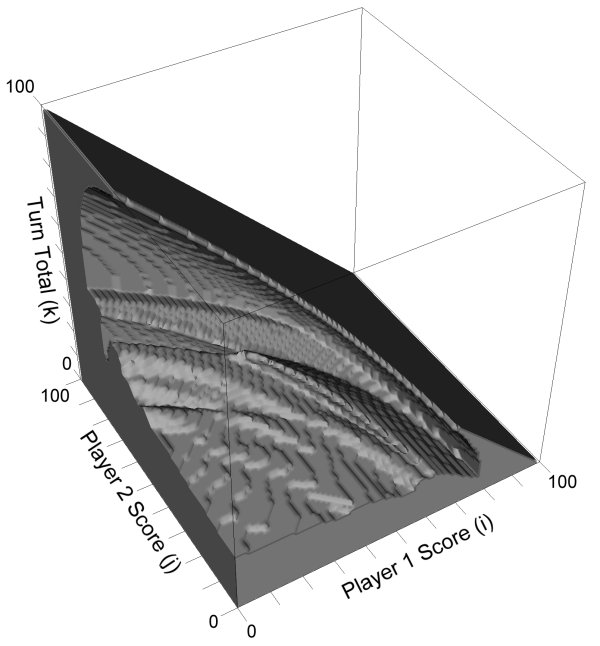
\includegraphics[width=0.5\textwidth]{neller_optimal_solution}
\caption{Roll\slash hold boundary for the optimal Pig play policy (Neller)\label{figure1}}
\end{figure}
\begin{figure}
\centering
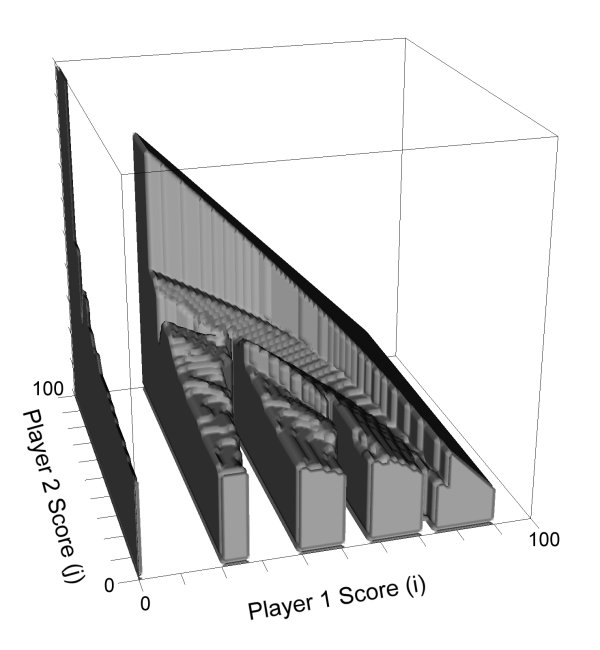
\includegraphics[width=0.5\textwidth]{neller_optimal_solution_2}
\caption{All of the states reachable by an optimal player (Neller)\label{figure2}}
\end{figure}

\subsection{Optimal strategy}
An optimal strategy is the strategy that, when played against all other strategies, is the best all-rounder. It will beat most others more than half the time, but may have a few weaknesses. As an example, in a game of rock, paper, scissors, the optimum is to play each of the three choices about a third of the time. However, in some game \textbf{[what does this mean?]} the optimum is to do something destructive. The optimum is not set out to get the best win ratio but instead it wants to minimise the maximum loss an opponent can impose on it.
\\
\\
One of the papers that T. Neller has published looks at finding the optimal strategy for Pig. As such the program \textbf{[needs explanation]} looked at all possible game-states within the Pig dimension and at each node picks the one with the highest win likelihood. In exploring this, we sought to reach Neller's optimal strategy using our own approach or, ideally, find a strategy that surpasses it.
\\
\\
Another possible outcome when looking into the optimal strategy (or optimal strategies) is that we find a pair of strategies that, when played against one another, exist in a Nash equilibrium. A Nash equilibrium (named after John Forbes Nash Jr.***Citate instead) is a point in a game space at which two strategies have to get worse against their opponent in order to adapt from their current position. Because of this, it would not be optimal to follow such a path so they remain in that state. This situation is demonstrated well in the prisoner's dilemma. It is defined as the following: \ \textit{If player A confesses and player B fails to confess, then player A goes free. If player A fails to confess but player B confesses, then player A will be convicted and sentenced for the maximum term in jail and player B goes free. If both players confess, then both players will be convicted, but the maximum sentence will not be imposed. If neither player confesses, both players will be framed for another crime in which a conviction is certain.}
\\
\begin{figure}
\centering
\includegraphics{prisoners_dilemma}
\caption{Prisoners' dilemma diagram \textbf{Is there a more specific caption we can use?}\label{figure3}}
\end{figure}
We can see from this diagram that the best outcome for each player is not to confess. However this is when one prisoner would look and say that confessing is the better option for them and then does so. Because this scenario is played such that both prisoners cannot discuss it then they would both make this discussion and you are left with the top left box after just a quick step. As you can see, this is not the best outcome for each of them, but they would have to take a greater loss in order to reach the best outcome and so are stuck in this Nash equilibrium.
\subsection{Preliminary findings}
The first step we took to familiarise ourselves with Pig was to do some tests of the game . We began by testing a few basic strategies, such as 'Bank at $20$'. We then tried to formulate our own strategies in an attempt to beat the aforementioned strategies. We were very successful in beating the previously defined strategies, which led us to believe that there are many strategies that in theory would be optimal but in practice are easily beaten.\\ \\Next, we started testing strategies on MATLAB using a script to simulate thousands of games between two strategies. R. Kniza theorised that banking at $20$ would be one of the most optimal ways to play in 'Dice Games Properly Explained'. However, we were quickly able to show that this was false, given that it was a worse strategy to play than 'Hold at $21$'. \textbf{[Is this true?]} Even though it was a marginal victory it was enough for us to be sure it was a better strategy.
\\
\\
These findings highlighted that there are many ways to perceive what an optimal strategy may be. However, without extensive testing, we did not know if these hypothetical optimal strategies could be beaten easily.
\subsection{Human Interactions in Pig}
Maximising the probability of winning can be determined through the use of MATLAB, as discovered by Todd Neller \textbf{[reference here]} to create an optimum solution. However, through the analysis of playing Pig ourselves, we discovered the human behavioural aspects that occurred during the game.
\\
\\
While a computer acts completely rationally, humans do not always act completely rationally when playing. Therefore, another aim of our project was to investigate how humans play Pig. This irrational behaviour is explained by a branch of economics called behavioural economics. Behavioural economics explains that not all actions taken are purely rational and a good part of what drives peoples thinking is purely social in nature. For example, when playing Pig humans are influenced by other aspects such as how well they are doing at a particular game-state compared with their opponent and their own risk preferences.
\\
\\
Thus, intrigued by these ideas, two experiments were performed to investigate the aspects of human interaction and behaviour during Pig. These were as follows:
\begin{enumerate}
\item Do players align game play with stated risk preference?
\item How are players' strategies influenced by their opponents'?
\end{enumerate}
The first investigation divided players into three categories: risk-averse, risk-seeking and risk-neutral. The other investigation looked into behavioural changes that occurred within a game. Modelling the strategic interaction between the two players allowed us to analyse behavioural patterns (since the game involves known payouts and quantifiable consequences). This allowed us to apply our understanding of game theory to help determine the most likely outcomes.

\subsubsection{Game theory and Nash equilibria}
Defined as the study of mathematical models of conflict and cooperation between intelligent rational decision-makers \cite{roger1991game}, the concepts within game theory provide a language to formulate, structure, analyse and understand strategic scenarios.\cite{turocy2001texas}
\\
\\
The underlying assumption within game theory is that the player – the individual who makes the decisions – is playing rationally. In this case, rationality is said to be achieved when the player seeks to play in a manner that maximises their own payoff. In the case of Pig, this is the first to bank to a certain number.
\\
\\
In 1950, John Nash demonstrated that finite games have always had an equilibrium point, whence all players choose actions which are best for them given their opponent. We analysed this through the monitored behaviour of player A vs player B.
\subsubsection{Player A vs Player B}
A key concept during the game play of Pig is dominance. No rational player will choose to play a dominated strategy (that is, a strategy which can be dominated by another strategy in all scenarios) since the player will always be better off when changing to the strategy that dominates their opponent. The unique outcome in the game will therefore be dependent on both players' strategies to find the maximising strategy. The two players may each have optimal strategies but when played together they don’t work since they have a negative impact on each other.
\subsubsection{Risk preferences}
For our second investigation, \textbf{[This is the ``first investigation'' above - might need to be re-ordered]} we focussed on the chosen risk preference stated by each player and compared it to how they actually play Pig.
\\
\\
Risk can be defined as the intentional interaction with uncertainty, and individuals differ greatly in their attitudes towards risk.\cite{what_is_risk_2017}
\\
\\
People differ greatly in their attitudes towards risk. Most individuals would, in general, prefer to take a less risky option when given a choice – they are risk-averse. However, some individuals prefer risk – risk-seekers, and some are indifferent towards risk and are considered risk-neutral. A risk-averse person will usually prefer a sure thing to a gamble where both have the same expected value. Conversely, a risk-seeking individual will try to choose a fair gamble over a sure thing; where a fair gamble is defined as a gamble with an expected payoff equal to that of a sure thing. Sometimes it happens that a risk-seeking person will end up choosing an unfair gamble (where the expected payoff is less than zero). Finally, a risk-neutral individual prioritises the option with the highest expected monetary value.
\\
\\
We can apply these risk preferences to Pig as follows:\\A risk-seeker will roll a greater amount of times on each turn and therefore bank on higher scores. A risk-averse individual will roll a fewer number of times at each turn and bank at lower scores and a risk-neutral player will be somewhere in between these two.
\\
\\
These three risk preferences are represented graphically in figure \ref{figure4}. On the $x$-axis is the payoff and on the $y$-axis is the expected utility.
\\
\\
\begin{figure}
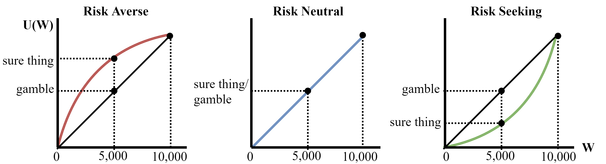
\includegraphics[width=\textwidth]{lottery-a-5}
\caption{risk preferences graph\label{figure4}}
\end{figure}
We wanted to see how an individual’s stated risk preferences affected their strategy when playing ‘Pig’. This information could then be used to calculate the optimal strategy for each of the three risk preferences. Over time, a computer could then adapt its strategy to find an optimal strategy for a player’s risk preference.

\subsection{Statisical analysis}
In terms of statistical analysis, we wanted to test whether or not a strategy is better than the one it is playing against based on the games they play against one another, given as a probability of winning. Firstly, we needed to establish what we believed to be a fair test between two strategies and the importance of this to our project. We approximated playing two strategies against one another to a statistical distribution and then constructed a confidence interval, at a particular level of significance, and then worked backwards by assuming that a strategy should beat itself with probability $0.5$. From this, we intended to find the optimal number of games required to run one single test between any two strategies, so that we could accurately say whether or not a particular strategy is consistently better than another.
\\
\\
After this had been determined, the next step was to decide the number of tests required to run in order to gain a desired degree of accuracy. Through this we were able to produce an accurate approximation \textbf{[bit of an oxymoron... maybe ``good approximation''?]} of the probability that one of each strategy winning with the player going first alternated on each trial. If this probability lies above the upper bound of the confidence interval, then the particular strategy could be declared better than its opponent. Similarly, a probability falling below the lower bound indicated that it was worse. However, if the probability fell inside the confidence interval, the two strategies were considered inseparable at our given level of significance, meaning we could not strictly say that one is better than the other.
\\
\\
\textbf{[future tense again - did we ever do this?]} We will then apply this in the same way to outcomes from our optimal strategy against other strategies. Hopefully, we can show that this such strategy is superior to other simple strategies before comparing to those that are more complicated such as Neller’s optimal strategy. Then, we hope to see if our optimal strategy has converged to that of Neller’s by the two being inseparable, after running the tests, at the given level of significance.

\section{Methodology}
\subsection{Group organisation}
Mia
\subsubsection{Meetings}
\subsubsection{Creation of project plan}

\subsection{Understanding the equations}

As discussed briefly in the introduction, linear equations can describe the probability of winning from any given game-state. This is a powerful method of calculation that Neller used to produce his optimal and we used for all of the programmed strategies we produced. As in the introduction, we let $P_{i,j,k}$ denote the probability of player A winning from the game-state $i,j,k$.
\\
\\
Firstly, let us look at the probability of A winning when banking. A is passing to B's turn by banking. So $P^{bank}_{i,j,k}$ will be equal to the probability A has on B's turn. The probability $Q_{j,i,k}$ is the probability the player B has of winning \textit{on their turn} at their game-state $j,i,k$. As Pig will have that either player will always win, so long as the game is finite, the sum of the probabilities from both players at any point in the game will be $1$. Note that this is from any point in the game, not at any game-state, as a game-state is specific to a player. From this we conclude that when it is player B's turn at game-state $j,i,k$, player A will have a probability of winning that is $1-Q_{j,i,k}$. By banking, A adds their turn score to their banked score, and B's turn starts with a turn score of zero. Thus we can define the probability A has at any game-state by banking as

\begin{align*}
P^{Bank}_{i,j,k} = 1-Q_{j,i+k,0}
\end{align*}

Take the probability of A winning when rolling.

\begin{align*}
P^{Roll}_{i,j,k} = \dfrac{1}{6} (1-Q_{j,i,0}) + \dfrac{1}{6}\sum^{6}_{r=2}P_{i,j,k+r}
\end{align*}

The first part on the right-hand side of the equation is when a $1$ is rolled. Similarly to banking, when a $1$ is rolled the game passes to B so the probability will be in terms of $Q_{j,i,0}$. The main difference is that the turnscore is not added to the banked score, as can be seen in the game-state, and there is only a $\frac{1}{6}^\text{th}$ chance of it happening. The second part on the right-hand side is the sum of all the other possibile outcomes of rolling. Again, each possible outcome has a $\frac{1}{6}^\text{th}$ chance of happening. The results take A to new game-states, with a higher turn score. $r$ represents the different scores that can be added, ranging from $2$ to $6$ depending on the number rolled.
\\
\\
How do we find out the useful probabilities that we have produced notation for? To explain it clearly, we will look at trivial probabilities and very simple calculations. The following equation gives the probability of winning from the game-state where the banked score of player A is 100. By the rules of the game, A has won, meaning this probability is equal to $1$.

\begin{align*}
	P_{100,0,0}=1
\end{align*}

This is one of many trivial gamestate probabilities that are important to understand. Another would be

\begin{align*}
	P_{82,0,20}=1
\end{align*}

In this case, player A has accumulated enough turn score to immediately bank and win. Generally, if $i+k\geq100$ and $j<100$ then the probability of that game-state is $1$, as it means the player has won. On the other hand, take the following game-state probability from A's perspective.

\begin{align*}
	P_{99,100,0}=0
\end{align*}

This game-state is where the opponent has won the game, so player A has $0$ probability of winning. Generally, if $i<100$ and $j\geq100$, then the probability at that game-state is $0$, as it means the other player has won.
\\
\\
These trivial game-state probabilities allow us to calculate the non-trivial probabilities of a game, which we will look at next.

\subsubsection{Simultaneous equations}
Let us start with a simple pair of equations, near the very end of the game. Both of the players are on $99$ points, and it is the beginning of player A's turn. Let us assume that both A and B roll on game-state $99,99,0$. It may seem an obvious choice, as they have no turn score to lose, but the idea of banking on a turn score of zero is something we shall be investigating further.

\begin{align*}
	P_{99,99,0} &= \frac{1}{6}\bigg((1 - Q_{99,99,0}) + P_{99,100,2} + P_{99,100,3} + P_{99,100,4} + P_{99,100,5} + P_{99,100,6}\bigg)
\end{align*}

From what we know about trivial probabilities, we see that if A successfully rolls, i.e. doesn't roll a 1, they win the game. So we can write the probabilities as followed, filling in the trivial probabilities.

\begin{align*}
	P_{99,99,0} &= \frac{1}{6}\bigg((1 - Q_{99,99,0}) + (1) + (1) + (1) + (1) + (1)\bigg)\\
	P_{99,99,0} &= \frac{1}{6}(1 - Q_{99,99,0})+\frac{5}{6}\\
	P_{99,99,0} &= 1 - \frac{1}{6}Q_{99,99,0}
\end{align*}

Similarly, for B's turn:

\begin{align*}
	Q_{99,99,0} &= \frac{1}{6}\bigg((1 - P_{99,99,0}) + Q_{99,100,2} + Q_{99,100,3} + Q_{99,100,4} + Q_{99,100,5} + Q_{99,100,6}\bigg)\\
	Q_{99,99,0} &= \frac{1}{6}\bigg((1 - P_{99,99,0}) + (1) + (1) + (1) + (1) + (1)\bigg)\\
	Q_{99,99,0} &= \frac{1}{6}(1 - P_{99,99,0})+\frac{5}{6}\\
	Q_{99,99,0} &= 1 - \frac{1}{6}P_{99,99,0}
\end{align*}

Now the two equations can be solved simultaneously, giving the results:

\begin{align*}
	P_{99,99,0} &= \frac{6}{7}\\
	Q_{99,99,0} &= \frac{6}{7}
\end{align*}

This example is one complete set of simultaneous equations. It turns out that every probability can be collected into a set of equations to be calculated. Whereas this one only contained two unknowns to be solved together, others may be much larger. A more complex simultaneous set can be seen if we start from A's turn at game-state $97,99,0$. Let A's strategy be to roll at this game-state.

\begin{align*}
	P_{97,99,0} &= \frac{1}{6}(1 - Q_{99,97,0})+\frac{1}{6}P_{97,99,2}+\frac{4}{6}\\
\end{align*}

After writting this out, we see the other probabilities it relies on. The method now is to see what the strategies do at these game-states and then write out the probability equations for them. In this example, let A roll at $97,99,2$ and B roll at $99,97,0$

\begin{align*}
	P_{97,99,2} &= 1 - \frac{1}{6}Q_{99,97,0}\\
	Q_{99,97,0} &= 1 - \frac{1}{6}P_{97,99,0}\\
\end{align*}

Now we have all three simultaneous equations that can be solved.

\begin{align*}
	P_{97,99,0} &= 0.8325\\
	P_{97,99,2} &= 0.8565\\
	Q_{99,97,0} &= 0.8612
\end{align*}

This looks good so far! Does this mean we can run through all the sets of equations now? Not just yet! \textbf{[ok Anthony chilll xD]} Firstly we must look at the interesting case of banking. Say for example instead of rolling at $97,99,2$, A banks. The equations are now:

\begin{align*}
	P_{97,99,0} &= \frac{1}{6}(1 - Q_{99,97,0})+\frac{1}{6}P_{97,99,2}+\frac{4}{6}\\
	P_{97,99,2} &= 1 - Q_{99,99,0}\\
	Q_{99,97,0} &= 1 - \frac{1}{6}P_{97,99,0}\\
\end{align*}

We do not need to write out the equation for $Q_{99,99,0}$ because we already calculated it in our first example. Its value was $\frac{6}{7}$. So with this we can again solve the equations, getting a much different result.

\begin{align*}
	P_{97,99,0} &= 0.7102\\
	P_{97,99,2} &= 0.1429\\
	Q_{99,97,0} &= 0.8816
\end{align*}

From this we conclude that when a strategy banks, it relies on knowledge of the probabilities of game-states nearer the end of the game than itself, which we shall call "higher game-states". Note that it will not rely on game-states "lower" than it as the game will always be progressing forward and a player cannot lose banked points. As long as we solve the sets containing higher game-states first, we can to run through and solve them all successfully.
\\
\\
Solving these equations means we can calculate every probability of winning from every game-state for any given strategy. Actually doing these calculations by hand is a ridiculous task however. Computational power is required to give us the probability values we want to calculate. This is where we turn to MATLAB for assistance.

\subsubsection{Matrices}
To make use of MATLAB, we needed to write the equations in terms of matrices. Every set of equations can be written in the form $CX=D$, where $C$, $X$ and $D$ are matrices containing the coefficients, the probabilities, and the constant values respectively. To see how these matrices are built, we will look at the examples used above.
\\
\\
The first important part is to simplify the equations. We want them in terms of separated probabilities and their coefficient values on the left-hand side of the equation, and a combined constant value on the right. This usually involves expanding brackets and adding constants together.\\ \\ We have:

\begin{align*}
	P_{99,99,0} &= \frac{1}{6}\bigg((1 - Q_{99,99,0}) + 1 + 1 + 1 + 1 + 1\bigg)\\
	Q_{99,99,0} &= \frac{1}{6}\bigg((1 - P_{99,99,0}) + 1 + 1 + 1 + 1 + 1\bigg)\\
\end{align*}

This becomes:

\begin{align*}
	P_{99,99,0} + \frac{1}{6}Q_{99,99,0} &= 1\\
	Q_{99,99,0} + \frac{1}{6}P_{99,99,0} &= 1
\end{align*}

Using basic ideas of matrix multiplication, we can construct a matrix,

\begin{align*}
	\begin{bmatrix}
	    1          & \frac{1}{6}\\
	    \frac{1}{6} & 1
	\end{bmatrix}
	\begin{bmatrix}
		P_{99,99,0}\\
		Q_{99,99,0}
	\end{bmatrix}
	=
	\begin{bmatrix}
		1\\
		1
	\end{bmatrix}
\end{align*}

This is useful as we can now take the inverse of the coefficients matrix, using it in left matrix multiplication to find the probabilities.

\begin{align*}
	C^{-1}CX &= C^{-1}D\\
	X        &= C^{-1}D
\end{align*}

Matlab has a function that does this for us, giving the probability values in the matrix $X$. Looking at the other two examples:\\
A rolling on $97,99,2$.

\begin{align*}
	P_{97,99,0} + \frac{1}{6}Q_{99,97,0} - \frac{1}{6}P_{97,99,2} &= \frac{5}{6}\\
	P_{97,99,2} + \frac{1}{6}Q_{99,97,0}                          &=  1\\
	Q_{99,97,0} + \frac{1}{6}P_{97,99,0}                          &= 1\\
	\begin{bmatrix}
		1           & \frac{1}{6} & -\frac{1}{6}\\
		\frac{1}{6} & 1           & 0\\
		\frac{1}{6} & 0           & 1\\
	\end{bmatrix}
	\begin{bmatrix}
		P_{97,99,0}\\
		P_{97,99,2}\\
		Q_{99,99,0}
	\end{bmatrix}
	& =
	\begin{bmatrix}
		\frac{5}{6}\\
		1\\
		1
	\end{bmatrix}
\end{align*}

A banking on $97,99,2$.

\begin{align*}
	P_{97,99,0} - \frac{1}{6}P_{97,99,2} + \frac{1}{6}Q_{99,97,0}) &= \frac{5}{6}\\
	P_{97,99,2}                                                    &= 1 - Q_{99,99,0}\\
	Q_{99,97,0} + \frac{1}{6}P_{97,99,0}                           &= 1\\
	\begin{bmatrix}
		1           & \frac{1}{6} & -\frac{1}{6}\\
		0           & 1           & 0\\
		\frac{1}{6} & 0           & 1\\
	\end{bmatrix}
	\begin{bmatrix}
		P_{97,99,0}\\
		P_{97,99,2}\\
		Q_{99,99,0}
	\end{bmatrix}
	& =
	\begin{bmatrix}
		\frac{5}{6}\\
		1 - Q_{99,99,0}\\
		1
	\end{bmatrix}
\end{align*}

Notice how $Q_{99,99,0}$ is in the constant values matrix. As discussed before, this is because its value will have already been calculated from a previously solved simultaneous set.

\subsubsection{Piglet}
To simplify the task, we first attempted to construct the matrices for a variant of Pig known as Piglet. In this game, players take it in turns to flip a coin until either a tail is flipped, or the player banks their turn score.
\\
\\
This simpler game contained all the same elements as Pig but on a smaller scale. Plainly, it is played with a coin rather than a die, so that probabilities are generated by $\frac{1}{2}$ , instead of the $\frac{1}{6}$ given by a die. The other difference is that you typically play to a much lower score than the $100$ in Pig. This score can be chosen to be whatever we want, often $10$ but sometimes as low as $2$ or $3$ for the most simple games.
\\
\\
A subtle yet vital difference is that $1$ is added for a successful flip. Consider if the coin was a two-sided die, with $1$ and $2$ rather than tails and heads respectively. If it was the same as Pig, the face value of the roll would be added to the turn score, so $2$, not $1$. We know that it is not possible to gain $1$ in Pig from a roll, as $1$ is reserved for a loss. \textbf{[Not sure how relevant this bit is]} This leads to a long list of questions regarding the rules of Pig. What if instead of losing on a roll of $1$, it was a roll of $6$ that loses the turn score or any other number? This was one of many points throughout our project where we found other areas to investigate, but decided to stay focussed on our set goals. For now we accept that Piglet adds $1$ to the turnscore on a flip of a head.
\\
\\
With a coin you may only score $1$ per flip, meaning you must flip a minimum of $10$ times for you to reach your end goal. In Pig this is not the case, as you can roll anywhere from $2$ to $6$ points on a successful roll, giving you a minimum of $17$ rolls to achieve your goal. Having a change in the minimum number of flips allows luck to have a much greater presence in the outcome of the game, as we observed upon playing it ourselves.
\\
\\
Our goal was to find the probability of a strategy winning when going first. For a strategy A, the probability of winning is $P_{0,0,0}$, as this is the starting point of the game on A's turn. Piglet's simplicity made it the perfect first stepping stone to solving this.

\subsubsection{Handwritten notes}
We first played Piglet to a total score of $3$, taking strategy A as banking on a turn score of $1$ and strategy B as banking on a turn score of $2$. (Both strategies would bank by default as soon as they got to the winning score.) From this we wrote out all the simultaneous equations by hand. This starts at the set that considers the probability $P_{2,2,0}$ and $Q_{2,2,0}$ whereby each strategy wins on its next go, similar to our first example in Pig. Once we had these equations written in terms of matrices, we manually put them into MATLAB and got it to solve them. From this we worked down through all simultaneous sets to obtain the probabilities of each strategy winning from game-state $0,0,0$.
\\
\\
\textbf{[This paragraph doesn't really add anything]} We repeated this process for a game to total score $2$, which we probably should have done before we did it for a total score of $3$. We used the same strategies again; strategy A was to bank on a turn score of $1$; strategy B was to bank on a turn score of $2$, which is equivalent to rolling at every game-state, what we called "rolling to win". We achieved another answer which looked relatively correct. As a group we noticed a pattern at this point to which the number of sets of simultaneous equations is that of the total score squared. It was here we realised that working out piglet to $10$ would require $100$ sets of equations. This was would be too much time would be wasted and have a high chance of us making mistakes.

\subsection{Coding}
Once we had familiarised ourselves with the rules of the game, the equations, the matrices, and a few simple Piglet examples, we moved to MATLAB. The goal now is build general matrices for every simultaneous set, and to make use of MATLAB's computational power. Then we could solve thousands of simultaneous equations and find all the probabilites at each game-state. We also wanted to make use of variable inputs to compare any strategy to another, and generalise the program to accept different winning scores and dice probabilities.
\\
\\
Our first attempt at simply getting out ideas down as code was a very simplified calculation of Piglet. Although we coded in a dice probability variable that could be changed, the code only worked for a dice flip, and when the variable was set to $\frac{1}{2}$. It was also limited to taking in only Bank on strategies. %Explain what Bank on strats are
We could however run to any winning score.
\\
\\
By using the hand calculated simple Piglet probabilities, we could check to see if our coded matrices were correct and fix any bugs. We even found that we could use the MATLAB-produed matrices to correct our handwritten mistakes. \textbf{[What does this mean?]} Once this was working we had our first runnable code to get us going. We just had to fully generalise the code. There were two steps to doing this: taking any strategy as an input, and having any dice probability working in the code. The former was easier; an independent problem that we made a function to do for us. The later was a little trickier but was a fundamental part of building the matrices.

\subsubsection{Strategies to matrices}
In our introduction, we defined a strategy as a 3 dimensional array of choices. Another way, and the way that we were introduced to strategies, is by a matlab function. These functions take inputs of "my score","your score", and "turn score", then output a "choice" that is a logical value of $1$ or $0$. Below is an example of Bank on 20.

% Inset Bank20 code

This way of defining a strategy was used when running the code for the game pig, which called the function strategies within it. However, it limited the way that more abstract strategies could be represented. Take a strategy that rolls in very specific locations for example, the function strategy would have to include many if statements to handle this, leading to a very big and hard to read function. An array of choices on the otherhand would always be the same size, and importantly it is easy to change if we wanted to. It is easy to locate the choice at a given gamestate too.
\\
\\
It makes sense to work with matrix strategies, but we still wanted to use function strategies in our code if we wanted to. So we devised a function \textit{Strategies to Matrices} that could convert functions to matrices but leave the strategy alone if it is already a matrix. First of all checked that the input was a function handle, then it runs through every gamestate, outputting the choice that the function produces, then stores that value in the corresponding matrix. We also used this function to check that the Matrix was the correct size for the game. Unlike function strategies, the matrix strategies only work for a certain game length.

% Inset Strategies to Matrices code

This allowed us to check what the strategy wanted to do at any gamestate, which was important for the type of equation to use when building the matrices.

\subsubsection{Coding Matrices}

This section covers how to build general matrices for any set of similtaneous equations. First of all, we need to consider what Probability values realy on eachother to produce a single set. Take $P_{i,j,0}$ the probability of A winning at the begginning of their turn. Assuming A rolls (we will look at banking on 0 later), $P_{i,j,0}$ will rely on other probabilities. On a successful roll, the new probabilities have different turnscores $k$, but same banked score $i$ and $j$. On an unsuccessful roll, a new probability from B's perspective is required; $Q_{j,i,0}$. This has not been previously calculated as it is not from a higher gamestate, therefore must be considered. Continuing on from the probabilities from A's perspective that we must now also consider, they can either bank or roll again. If A banks, that probability will be equal to $1-Q_{j,i+k,0}$, where $k$ is the now non zero turnscore. As $Q_{j,i+k,0}$ is for a higher gamestate, it would have already been calculated, so there are no new probabilities to consider. Banking is an easy choice to deal with for this reason. If A rolls again at the new gamestates with a higher turnscore, more probabilities must also be considered. The important fact however is that only the turnscore has changed again. They also rely too on $Q_{j,i,0}$ if the roll is unsuccessful, which is one we are already considering. It seems then that we must consider all $P$ probabilities containing a higher turnscore but the same banked scores, as our orignial $P_{i,j,0}$, up until the turnscore has won A the game.
\\
\\
We have only considered $P$ probabilities from A's perspective so far, but we also rely on $Q_{j,i,0}$. Similarly to what we have discussed with repects to A's probabilies $P$, we must consider all $Q$ probabilities with higher turnscores up until the turnscore has won B the game. Again however, only the turnscore is changing. It can be concluded then that each set of similtaneous equations is built around fixed banked scores $i$ and $j$. This fact could also have been reached by realising that any higher game state (higher banked values) than the current one would have already been calculated so would not produce another equation, and no lower game state (lower banked values) would ever be called because the players cannot loose banked score.
% This is kind of like a theorem that i have just proved
% The main point of the last two pareagraphs was to prove "It can be concluded then that each set of similtaneous equations is built around fixed banked scores $i$ and $j$."
% How can we highlight that sentence to make it stand our as the whole point
\\
\\
From this % from theorem above
we see that there must be a similtaneous set for every banked score $i$ for A and every banked score $j$ for the opponent B. In the piglet section we explained how we noticed that the number of sets was the "to win" score squared. It is now clear to see why that is the case. $i$ and $j$ can take the same amount of values as the "to win" score so multiplying them together for every possible combination gives the "to win" score squared. This gives us some scope on how many sets will need to be solved in Pig... $100\times100\times100=1$ million.
\\
\\
Now we have a rough idea of every equation in any similtaneous set. For clarity, we will order them as follows in the probabilities matrix, $X$.
\begin{align}
	\begin{bmatrix}
		P_{i,j,0}\\
		P_{i,j,1}\\
		...\\
		P_{i,j,n-1}\\
		P_{i,j,n}\\
		Q_{j,i,0}\\
		Q_{j,i,1}\\
		...\\
		Q_{j,i,m-1}\\
		Q_{j,i,m}\\
	\end{bmatrix}
\end{align}
where $n=\text{"to win score"}-i-1$ and $m=\text{"to win score"}-j-1$.
\\
\\
The first problem to our assumptions so far is that we will need all of these equations. This only outlines all of the ones that could be needed. Take for example, the set built around $0,0$, where A is banking on $20$. $P_{0,0,50}$ for example would never be considered, as the strategy would have banked many rolls ago. For banking on 20 strategy, the gamestate $0,0,50$ and many others would be impossible. This idea of impossible gamestates was touched on in the introduction, the difference here is that this one is specific to a strategy. As discussed in the introduction, a turnscore of 1 is also not possible for pig.
\\
\\
This problem has a suprisingly elegant solution. The definition of an impossible gamestate is one that cannot be reached from other gamestates. The coefficient's matrix will be filled from top to bottom, meaning lower turnscore probabilities are completed first. So if we get to any probability that is an impossible game state, it would not have been called by any other gamestates before it. Therefore all the coefficient values for it would be zero. This is a simple to check in our program. We then go on to ignore this row of the matrix, which is the same as it not being there. With this problem solved, we can use the set probability matrix described above, without worrying if the probability is relevant or not.
\\
\\
Now we can fill in the coefficient matrix and the constant value matrix. This is done by checking what the strategy does at each gamestate, either rolling or banking. This is much easier with the matrix strategies. By making use of Matlab's variables, for loops and general programming techniques, we successfully put all the needed values into the matrices. We produced truly remarkable code for this function which this margin is too small to contain. % Banter
% Na seriously not sure if i should put the whole code in there, I think i've explained how it works pretty well without the code itself and that might confuse the reader
% Gonna put in a matrix example here though so that should do, including roll examples, bank examples, and impossible GS examples.
\\
\\
We then run through every gamestate backwards, collecting the probabilities as we solve them. Remember that matrices might need the probabilities calculated from higher gamestates, so  whilst we build our collection of probabilities, we will call upon them as we work down. Once we had completed every matrix calculation, we had a generalised working code that could calculate the probabilities of winning at any game state, for any two strategies, for any given dice proability and to any winning score.
\\
\\
For pig, Matlab completes all 1 million sets in 5 seconds, must faster than we could have by hand! Although we have every probability on Strategy A's turn $P_{i,j,k}$ and every probability on Strategy B's turn $Q_{i,j,k}$. The main outputs that we are interested in, is $P_{0,0,0}$ and $Q_{0,0,0}$; the probability each strategy has of winning, when going first.

\subsubsection{Testing the code}

% Rhodri

To test the output of the code, we compared the calculated probabilities to experimental results. It was sufficient to test only the value in the lowest position in the matrix, $P_{0,0,0}$, since this value relies on the higher game-states (and therefore any errors in higher positions should be reflected in this output).
\\
\\
$P_{0,0,0}$ represents strategy A's probability of winning at the start of the game, assuming strategy A is the first to roll. To test this value, we simulated a series of games of pig with strategy A always being the first to roll, and outputted the number of wins for strategy A. For example, our $P_{0,0,0}$ for the input strategies ``bank on 20'' and ``bank on 21'' was 0.542626, indicating that ``bank on 20'' has a 54.26\% chance of beating ``bank on 21'' when going first. Running 1,000 series of 1,000 games gave us a distribution for the number of wins for ``bank on 20'' displayed in figure %ummm number?
. The median on the boxplot is very close to the projected probability which indicated that our code had correctly calculated $P_{0,0,0}$.

% Figure goes here please Liam :)

We similarly tested some more simple strategies with successful results. Then we tried to create awkward strategies that would test the limitations of our program. Of special interest were strategies that involved banking at turnscore 0, i.e. ``skipping'' a turn. In certain circumstances this decision could theoretically lead to a stalemate, where both strategies refuse to roll. While this would never happen in practical play, it was important to equip our Matlab script to deal with these scenarios so that it wouldn't cause issues when we later come to computer-generated strategies.
\\
\\
A particularly interesting example is a strategy which skips a turn whenever the two players' banked scores are equal. (For convenience we exclude the starting game-state where both players have score 0.) When this strategy plays against itself, around a quarter of games result in stalemates. But because the majority of games resulted in victories for one player, we still wanted to be able to analyse this strategy, and therefore had to update the code to accommodate stalemates.
\\
\\
The goal was that a stalemate would be counted as a loss for both players, since this is not a desirable outcome for our optimal strategy. Our modification therefore had the entire code run twice if a stalemate was detected. On the first run, every stalemate was declared a victory for player B (hence a loss for player A) to give an accurate recording of $P_{0,0,0}$. On the second run, we reverse the order of the strategies so that stalemates are counted as a victory for player A (hence a loss for player B), giving us an accurate value for $Q_{0,0,0}$.
\\
\\
Adjusting the script for simulating series of games to output the number of stalemates, we could then accurately test the $P_{0,0,0}$ and $Q_{0,0,0}$ values for strategies involving skips. Now satisfied that our code gave reliable outputs for any input strategies, we were ready to use this script to compare optimal strategies.

\subsection{Behavioural Economics}
To investigate if players aligned game play with their stated risk preference and see if players were influenced by how well their opponent is doing, we decided to get a sample of people from the ECM3735 (Mathematical Group Project) module to play pig. We gathered 15 samples, which was 15 games played with 30 people’s risk preference and game strategies gathered.
\subsubsection{Method}
\begin{enumerate}
\item Contacted Barrie to ask if we would be able to use time in our drop-in sessions to get students to participate.
\item Created a tracker form, figure \ref{figure5}.
\item Purchased dice and printed off tracker form.
\item Explained to the participants how to play Pig to 100.
\item Explained to the participants to circle each of the three questions, without letting their opponent see (limits any chance of dependent preference choosing).
\item After each players go they had to write down the amount scored (bank score) and the amount of times they had rolled (No. of times rolled) allocated to each turn number (turn no.).
\item Each player did this until one player won.
\item Collected in the forms.
\item Inputted all the data into excel documents, categorising each player into one of the three risk preferences. Example shown in figure \ref{figure6}.
\item We calculated the accumulated scores for each player, and began our analysis – shown in findings (put section reference).
\end{enumerate}
\begin{figure}
\center
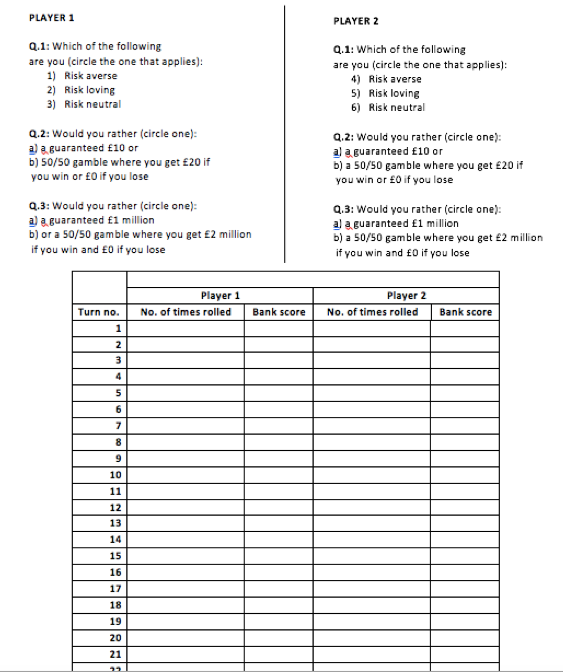
\includegraphics[scale=1]{pig_tracker_form}
\caption{`Pig' tracker form\label{figure5}}
\end{figure}
\begin{figure}
\center
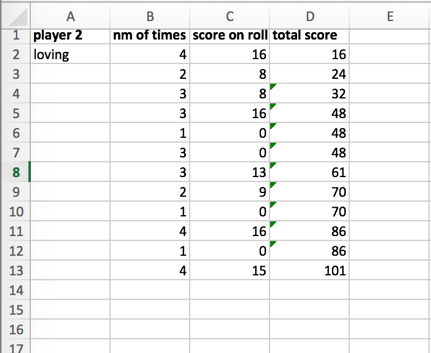
\includegraphics[scale=1]{excel_1}
\caption{Information inputted into Excel\label{figure6}}
\end{figure}
The reasoning behind the questions on the tracker form:\\
\textbf{Question 1}\\This question was used to find out participants risk preference (risk neutral, risk averse, risk seeking) so we could see if individuals actually stuck to their stated risk preference whilst playing.\\ \textbf{Questions 2 and 3}\\We created these questions to test whether this would correlate with the stated preference in question 1. The risk neutral person (in theory) should have no preference to option a or b as they both have the same expected payoff. A risk averse person (in theory) should pick option a in both cases and a risk seeking person will (in theory) pick option b in both cases. Both question 2 and 3 represent gambles, however the expected payoff in question 3 is much greater than that of question 2. Therefore question 3 allows us to see how risk seeking a participant may be, as a greater payoff will be a lot more attractive to a risk seeker.\\ \\These questions created were motivated by a branch of economics called Prospect Theory. As in Kahneman and Tversky’s 1979 paper, prospect theory is the ‘Analysis of decision under risk’\cite{kahneman2013prospect}. The theory explains that humans dislike losing far more than we like winning and that depending on whether a scenario is framed as win or a loss, we act differently. Humans dislike losing so much, that they are willing to take huge risks to avoid a loss scenario. As an example, in the case of ‘Pig’, if player A is close to winning and player B is far behind, then player B will usually try to keep rolling on their turn, to build up a big score and then bank it, when actually their optimal strategy might be to bank earlier on. (this is later discussed in REFERENCE)
\subsection{Statistical Testing}
\subsubsection{Fair test}
Throughout our project, we will be testing numerous different strategies against one another to determine whether a strategy is better than another. To do this accurately, we will need to ensure that the test we conduct is fair and will give a reliable result. This will be particularly important for our final findings when we want to test our version of the optimal strategy. We will want to know whether it is an optimal strategy or whether there are still some strategies that are able to beat it, meaning it isn’t `the' optimal.\\ \\To determine whether a strategy is better than another is not as simple as playing them against each other once and deciding that the winner is the better strategy. A strategy will have a theoretical probability of winning against another given strategy, but playing only one game may not give a reliable result. Say you were to play the same strategy against itself.  The theoretical probability of either strategy winning would be $0.5$, if you were to alternate which goes first and to play a numerous amount of games. By playing only one game you would deduce that one of the strategies is better than the other even though they are the same strategy. You could also play two strategies where one has a significantly larger theoretical probability of winning than the other, but the test could conclude that the worse strategy wins, meaning you would accept that the lesser strategy is better even though theoretically it is not. This false result will be due to statistical inference.\\ \\In the world of stats, theoretical probabilities don’t always agree with the practical results, though there are ways where you can improve the accuracy of a practical test to make it more accurate, closer to its theoretical probability. That is the point behind the fair test, to try and get a result that’s accurate to within a certain confidence of the theoretical results.  In our case, we can increase the number of games we play so that inference is reduced, therefore giving a reliable score when testing strategies.  Instead of playing only 1 game, we can play numerous games and then take scores. Say we played $100$ games, each individual game of pig will result in a winner which will result in that strategy receiving a score of $1$. This will be continued until $100$ games are complete and the probability for each strategy would be their score divided by $100$, in this case.\\ \\The true $n$ value will need to be calculated and not decided. To do so we can use hypothesis testing. From theoretical probability values, we can define an interval around the value for which we want the practical result to lie in. The practical test will involve playing $N$ amount of games of pig were a strategy receives a score of $1$ for each game they win. After $N$ games have been completed, we can calculate the probability of the strategy winning against the other by dividing the number of games it has won by the total number of games. Then we can test numerous results for different values of $N$ and observe the distribution of $p$ as $N$ increases. From there we can chose an appropriate value for the number of games which will give us constant results within our confidence interval. Once this value has been obtained, the testing of strategies should result in reliable results and therefore be as fair of a test as possible.
 \subsubsection{Deciding that a strategy is better than another}
As mentioned before, to decide that one strategy is better than another is not as simple as playing one game of pig and saying that the victor is a better strategy.\\ \\Once we have decided on a value for $N$ at which we decide that the test is fair, it will follow immediately what results will conclude that one strategy is better than another. By finding $N$, we will have chosen an upper and lower limit of the $p$-value at which we want our results to lie within. To illustrate this, say we conclude that $100$ games of pig is a form of a fair test and we want our practical probability to lie within $0.1$ of the true (theoretical) probability. If we were to test the same strategy against itself, theoretically either strategy should win with a probability of $0.5$, therefore after performing practical tests, we will want the representative probability to lie within $0.4$ and $0.6$. As the probability will be calculated by dividing the number of wins a strategy had and dividing it by the total number of games, we can then either perform this calculation to find the representative probability or we can calculate directly from the confidence interval how many games a certain strategy will need to win in order to conclude that it is a better strategy. In the above case, as it will need to have a probability higher than $0.6$ to conclude that it is a better strategy, it will therefore need to win $100\times0.6=60$ games at least in order to be considered a better strategy.
\subsubsection{Testing our optimal}
To finalise our findings we will need to test our version of the optimal to find whether it is actually an optimal or at least as good as Neller’s\citep{neller2004optimal}, therefore we will need to run some test on it and evaluate the findings.\\ \\We may begin our testing by playing our version of the optimal against simply hold at strategies, which have actually been found to be quite effective, even against Neller’s strategy:  Though of course, not better than it. By doing this we can decide whether it is actually better than simple hold at strategies or whether it needs adjusting before playing it against Neller’s version.\\ \\Throughout these test we will keep to our definition of whether a strategy is better than another. Once we have succeeded in deducing that our version is better than all hold at strategies, we may then test our version against Neller’s and analyse the results.

\section{Findings}

Anthony

\subsection{Pig}
\subsubsection{Did we solve Pig}

\subsection{Behavioural Economics}
\subsubsection{Do players stick to their stated risk preference}
To determine whether players stuck to their stated risk preferences, we divided all of the samples into the three risk preference categories (risk averse, risk seeking, risk neutral). After doing this, we plotted the total score of each player at each turn
\begin{figure}
\center
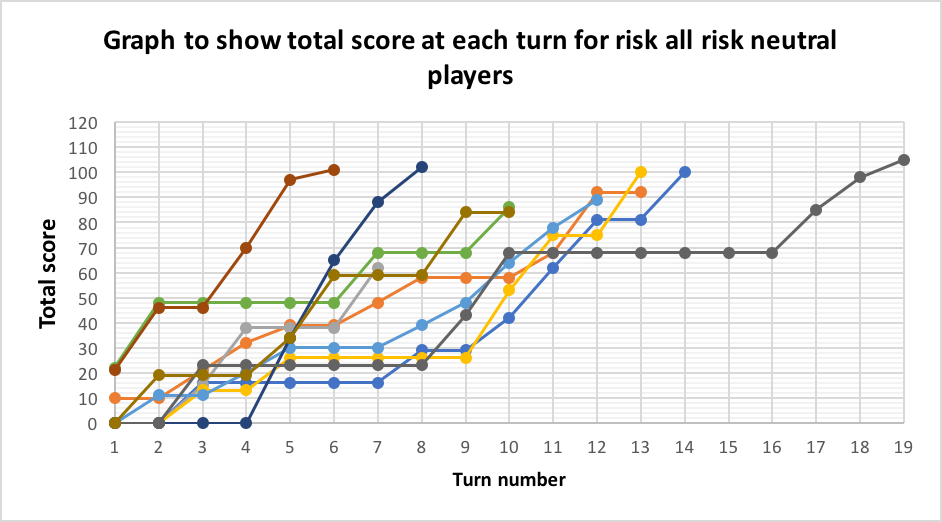
\includegraphics[scale=1]{neutral_graph}
\caption{Score at each turn for risk neutral players\label{figure7}}
\end{figure}
\begin{figure}
\center
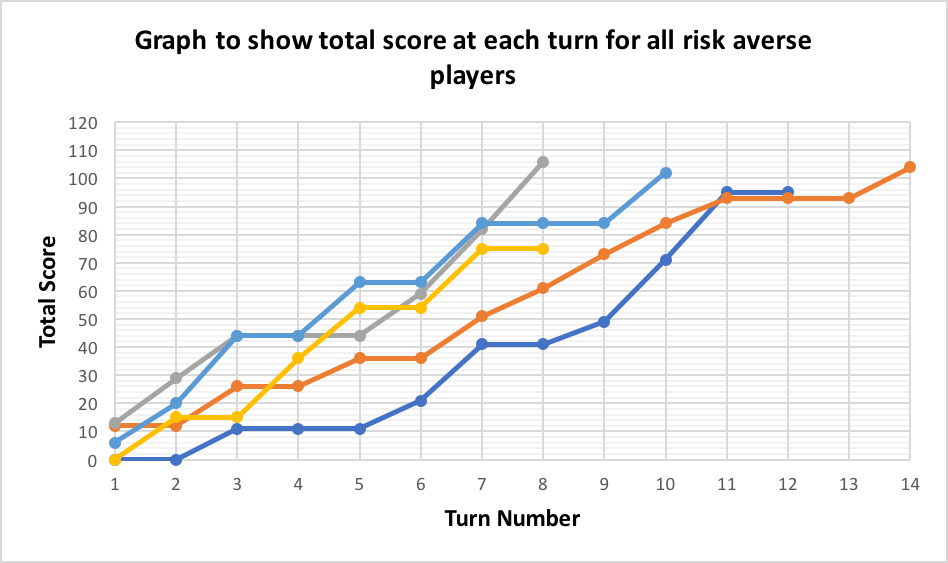
\includegraphics[scale=1]{averse_graph}
\caption{Score at each turn for risk averse players\label{figure8}}
\end{figure}
\begin{figure}
\center
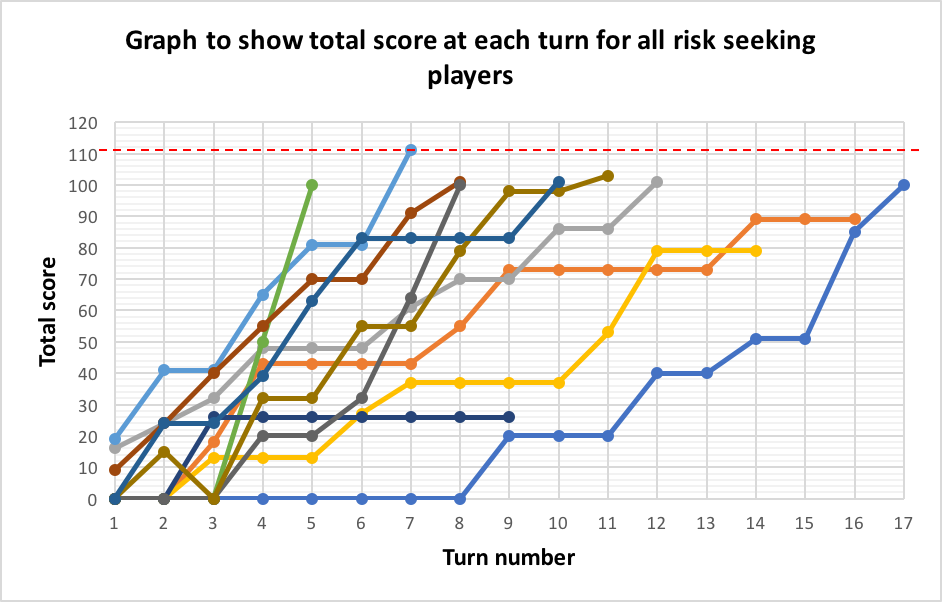
\includegraphics[scale=1]{seeking_graph}
\caption{Score at each turn for risk seeking players\label{figure9}}
\end{figure}
For all three of the graphs (figure \ref{figure7}, figure \ref{figure8}, figure \ref{figure9}) the plotted results are all fairly similar in shape and gradient, which we didn’t expect initially. So, to investigate further we decided to find the average total score at each turn number for each of the three risk preferences (figure \ref{figure10}, figure \ref{figure11}, figure \ref{figure12}).\\ \\
\begin{figure}
\center
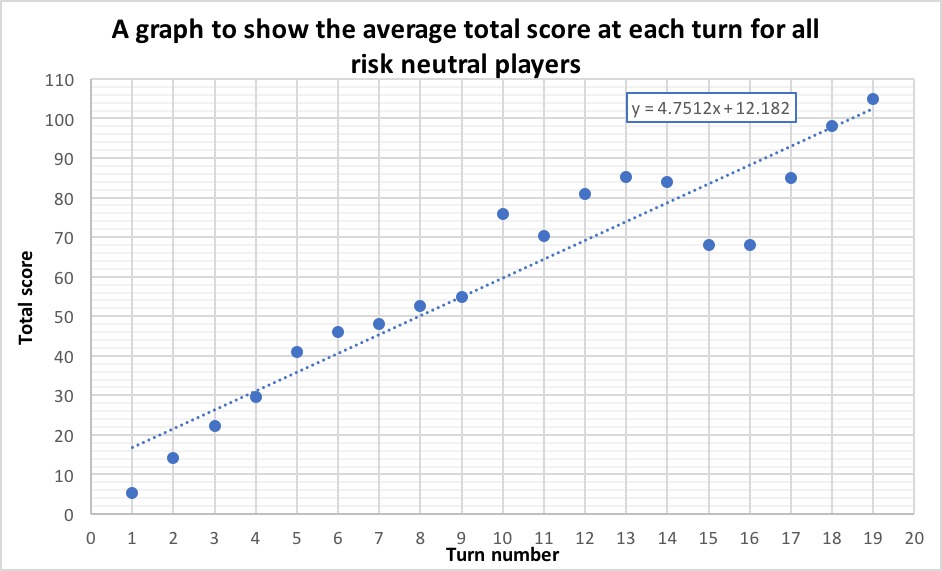
\includegraphics[scale=1]{average_neutral}
\caption{Average score at each turn for risk seeking players\label{figure10}}
\end{figure}
\begin{figure}
\center
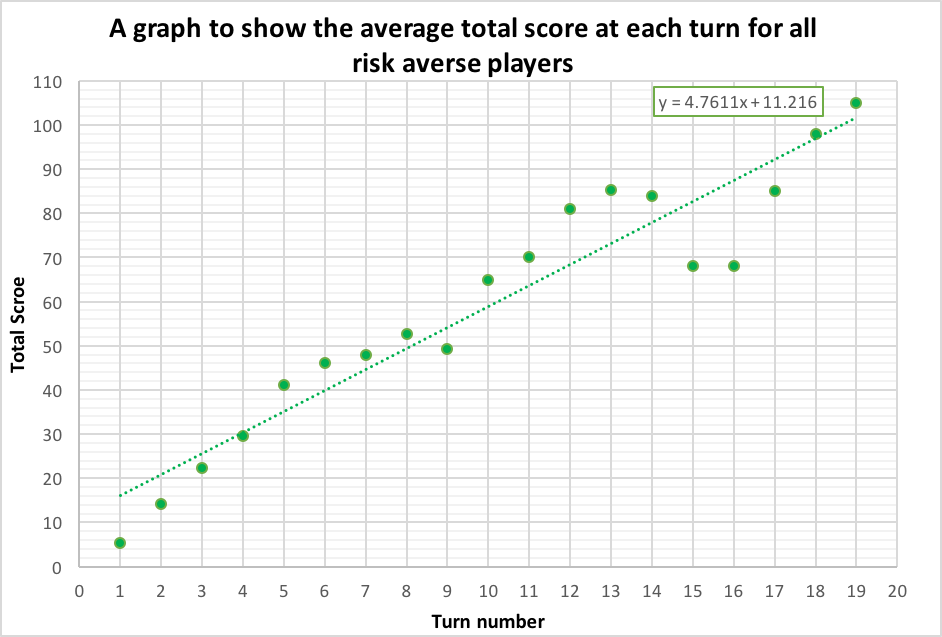
\includegraphics[scale=1]{average_averse}
\caption{Average score at each turn for risk seeking players\label{figure11}}
\end{figure}
\begin{figure}
\center
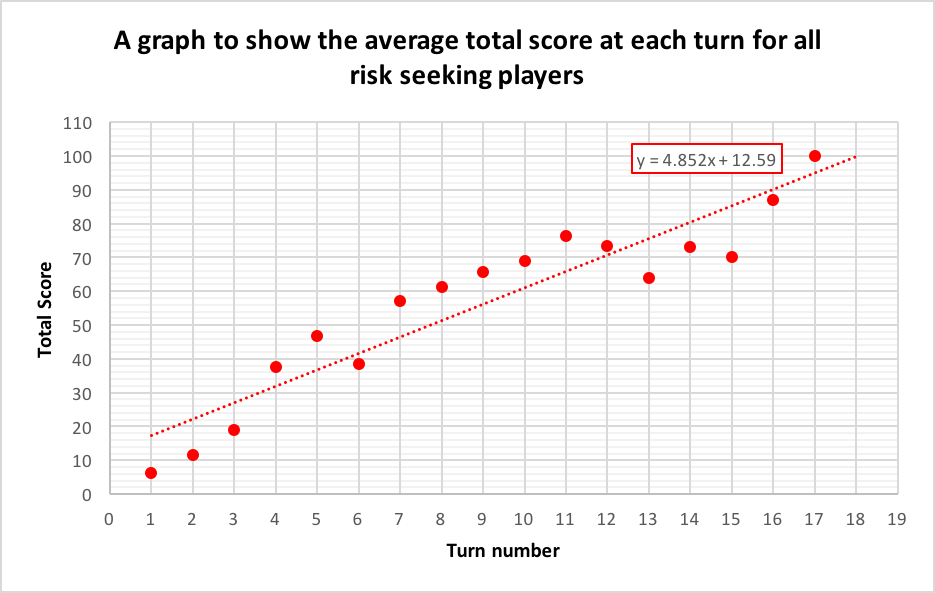
\includegraphics[scale=1]{average_seeking}
\caption{Average score at each turn for risk seeking players\label{figure12}}
\end{figure}
Looking at figure \ref{figure10}, \ref{figure11}, \ref{figure12}, we can see that they are actually all very similar. On further inspection of the gradients of the trend lines, we can see that the risk neutral average graph has a gradient of $4.75$, the risk seeking average graph has a gradient of $4.85$ and the risk averse average graph has a gradient of $4.76$.\\ \\The gradients are therefore all very similar. The results have shown that the gradient is greater for risk seekers than risk averse participants, however, we expected there to be a greater change in the gradients. This is because risk seeker’s would roll more each turn to increase the chances of a getting a high bank score. Whereas a risk averse participant would bank on a smaller score at each turn as this is a safer option.\\ \\A risk seeker would potentially believe the outcome of rolling and scoring a greater bank score would be of greater interest then banking at a safe score, therefore they would be at a greater risk of rolling a 1 and losing all the points from that round. This could therefore explain why the gradient is only a smaller percentage greater, as looking through the game strategies performed by risk seekers a lot of them banked on a score 0, due to rolling a greater amount of times thus a greater chance of scoring 1. Therefore their overall accumulated score was still achieved by the same amount of turn numbers as risk adverse participants.\\ \\In addition, we expected the risk neutral gradient to be equally between the risk seekers gradient and risk averse gradient. Conversely, it’s the lowest gradient of the three. This could be due to experimental error as the difference between the greatest and lowest gradient is only $2\%$.\\ \\Moreover, looking at all three graphs the points plotted at turn number 15-16 are all below the average gradient by a significant amount. This could be because at this point in the game the players opponent is close to winning and therefore the player begins to panic and roll too each turn number, causing them to roll a 1 and lose. This links back to the ideas exposed in Prospect theory as humans compensate to win by taking extra risks which they usually wouldn’t. In this case the player is rolling excessively in order to rebuild up a greater score to bank on. This therefore shows, that for our results gathered, that at around the turn number 14, on average, players strategies change dependent on the opponents play.\\ \\Overall, a possible explanation for the similarity of the gradients is that in the long run of playing pig, players preferences are ‘evened out’ by the game, much like the stock market evens out returns in the long run.
\subsubsection{Players Interactions}
For our second experiment we looked into how players A’s strategy was influenced by player B’s strategy and vice versa. To do this we took all 15 sample games that were played and plotted the total scores of player A and player B at each turn.\\ \\Firstly, an interesting game that we wanted to look at was game 14 (figure \ref{figure13}).\\ \\
\begin{figure}
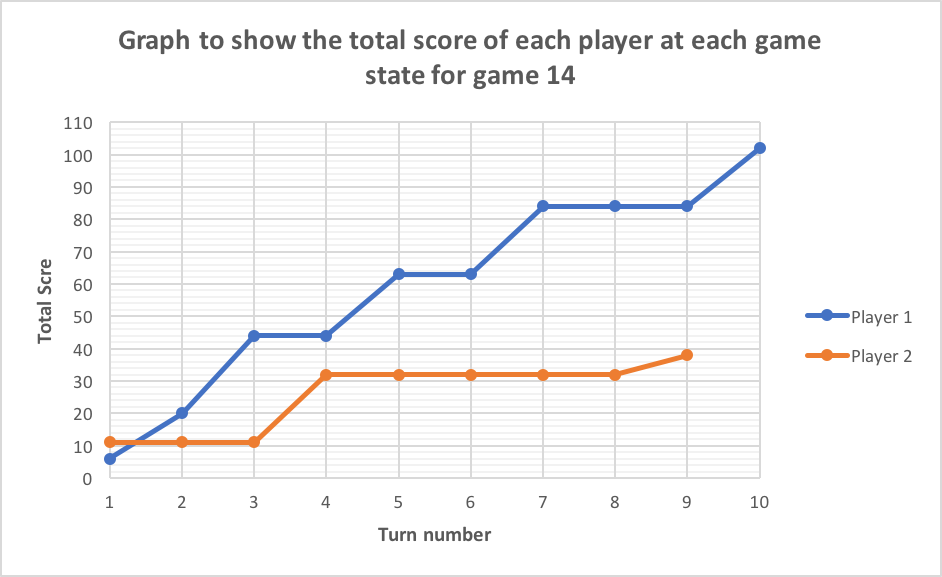
\includegraphics[scale=1]{game14}
\caption{Game 14 – Player 1: Risk Averse, Player 2: Risk Neutral\label{figure13}}
\end{figure}
Looking at game 14, we found that from turn 4 onwards, as player 1’s score increases and gets closer to the target score of 100, player 2’s total score stays the same until turn 8. A possible explanation for this is that as player 1 continues to increase their total score, player 2 wants to try and build up a big bank score in order to catch up with player 1. As a result, they’ve roll for too long, eventually rolling 1, thus scoring a turn total of 0.\\ \\This shows us that player 1’s strategy is influencing the strategy used by Player 2. At first, both players represent similar game techniques, but after an increased score from Player 1, Player 2 demonstrates traits of a risk seeker (although they stated to be risk neutral) by rolling a greater amount of times to attempt to gain a better outcome. However, in this case they have been unsuccessful. This highlights two concepts. Firstly, player 2 has not stuck to their stated risk preference during the game, and secondly, the strategy implemented by player 1 has resulted in a change of behaviour in player 2. As this game lead to a lose for player 2 it may show that a strategy shouldn’t be changed during game play, and that individuals should play a strategy that is independent of their opponents.\\ \\
\begin{figure}
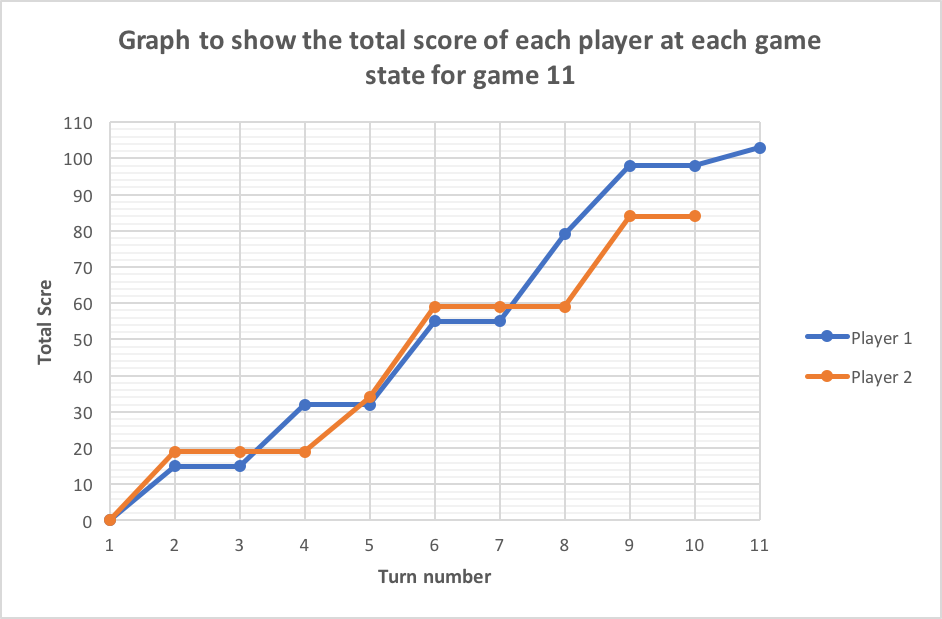
\includegraphics[scale=1]{game11}
\caption{Game 11- Player 1: Risk loving, Player 2: Risk Neutral\label{figure14}}
\end{figure}
Whilst looking through all of our results we found a common theme that is shown well through Game 11 (figure \ref{figure14}) in particular. We can see that players start to mirror one another’s strategies.\\ \\The stated risk preferences of each player are different and therefore we would expect slightly different graphs from each player. However, they both follow the same pattern from the beginning of the game. The shape of the graphs follow that of one expected by a risk neutral participant and thus may show that player 1 (stated risk loving) has actually adopted the strategy of player 2.
\subsection{Statistical Testing}
\subsubsection{The test}
As mentioned in the methodology, to calculate the number of games required to play to perform a fair test we will use hypothesis testing.\\ \\Let $S$ denote a certain strategy within the game of pig.\\ Let $n$ denote the number of games played.\\Let $X$ denote the number of games won by that strategy after $n$ games.\\ As we will be playing $S$ against itself, we can say $E(X)=\dfrac{n}{2}$, the expected amount of games $S$ should win against itself. \\We can approximate $X$ to the binomial distribution to conduct the hypothesis test. $X \sim Bin(n , p=0.5)$
by the binomial distribution
\begin{align}
E(X) &= np & SD(X) &= \sqrt{var(X)}\notag\\
&= \dfrac{n}{2} & &= \sqrt{np(1-p)}\notag\\
& & &= 0.5\sqrt{n} \notag
\end{align}
By using the $Z$ distribution at a 95\% confidence interval $(z=1.96)$, we compute the following interval.
\begin{align}
95\%Cl &= (\dfrac{n}{2} -1.96(0.5\sqrt{n}), \dfrac{n}{2} +1.96(0.5\sqrt{n}))\notag\\
&= (\dfrac{n}{2}-0.98\sqrt{n}, \dfrac{n}{2}+0.98\sqrt{n})
\notag
\end{align}
We would like the $p$ value that we obtain to be within $0.025$ of the true value of the probability. As probabilities range from $0$ to $1$, this would mean that the practical result is within $95\%$ of the theoretical value. For this system this implies that $0.475<p<0.525$. From the above interval for $X$, we can say that as $X=np$, using the upper and lower bounds for our $p$, we can then calculate a value for $n$, i.e. $0.475n$ would be equal to the lower bound for $X$ of the confidence interval with $0.525n$ being the upper bound.\\I.e.
\begin{equation}
0.475n=\dfrac{n}{2}-0.98\sqrt{n}
\notag
\end{equation}
Solving this for $n$, we get that $n=1537$, and similarly for the upper bound.\\ \\This would imply that playing a game of pig $1537$ times would end up giving a probability of the strategies winning against each other that is within 95\% of the true value. As theoretical stats is not 100\% accurate, this theory was simulated in matlab. We tested this theory by running $n$ games of pig $100$ times for a given strategy against itself, for $n$ ranging from $1$ to $4000$, and calculating the $p$-value from each of the games.\\ \\
\begin{figure}
\centering
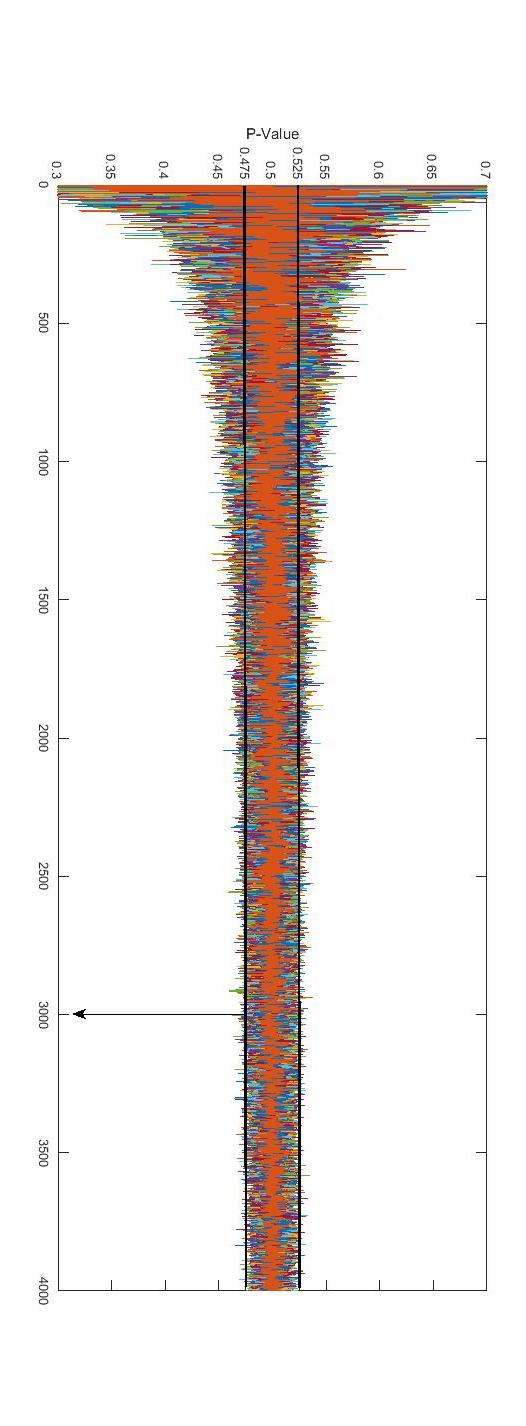
\includegraphics[height=24cm]{stats_testing}
\caption{stats testing\label{figure15}}
\end{figure}
Figure \ref{figure15} shows the distribution of the $p$-values over the number of games played. Each point on the $x$-axis has $100$ values for the $y$-axis. The two lines on the $y$ axis at $y=0.475$ and $y=0.525$ show the confidence interval we want for $p$. The orange colour that runs through the graph shows a higher concentration of values. This graph shows that the distribution for $p$ is scattered greatly for small number of games played and converges as the number of games increases. We can see that around the $1500$ number of games played, the orange centre is located within the interval for $p$, but there are still a lot of stray values. These stray values still occur, but less often, even when the number of games is increased. By looking at the graph we can chose a value at which the majority of points lie within the interval.\\ \\After the number of games passes $2500$, there doesn’t appear to be much decrease in the width of the distribution, so we will chose $3000$ as the appropriate number of games to play for a fair test. It would be a mistake to now only use $n=3000$ to test strategies. As the figure \ref{figure15} shows, even for high values for $n$, you can still get stray results. Therefore, like what was done in the test to find $n$, for strategies we want to compare we will take $100$ results of $3000$ games. Then we can take the average of these results to further improve the reliability of the result.
\subsubsection{Corollary}
\begin{figure}
\centering
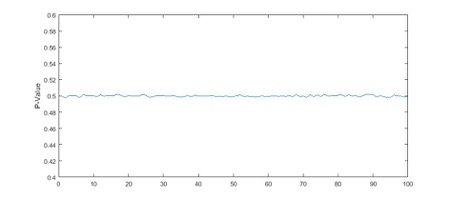
\includegraphics[width=\textwidth]{stats_2}
\caption{stats\label{figure16}}
\end{figure}
In matlab, we tested the fair test numerous times by creating a code which ran the test $100$ times, that is, $100$ results $3000$ games played $100$ times with the average computed. Figure \ref{figure16} illustrates $1$ of the results of running this code. You can see that for $100$ results of the test, the distribution of $p$ is still very small. For this particular result, $p$ ranged from $0.4974$ and $0.5020$ which is well within our confidence interval for $p$. The mean of the results was (coincidently) $0.5$ exactly.\\ \\The purpose of the fair test is that our practical results are accurate to within a certain degree of confidence to the theoretical results, in our case, within $0.025$. As we have coded a programme which can calculate the theoretical probabilities, we can run multiple simulations with the fair test to see how accurate our results are to the theoretical values.
\subsubsection{Testing theoretical probability values to practical values with the fair test}
We have showed that for a strategy playing against itself, playing $3000$ games $100$ times gives a reliable result for the probability of winning, but we now should ensure that this test also works for different strategies playing against itself. From using the theoretical probabilities calculated in matlab, we will run numerous tests for different strategies playing against themselves and comparing the theoretical results to the practical results obtained from the test. We will consider simple hold at strategies with this. Due to time constraints we will not compare every hold at strategy, though we will test a wide variety of hold at strategies.
\begin{figure}
\centering
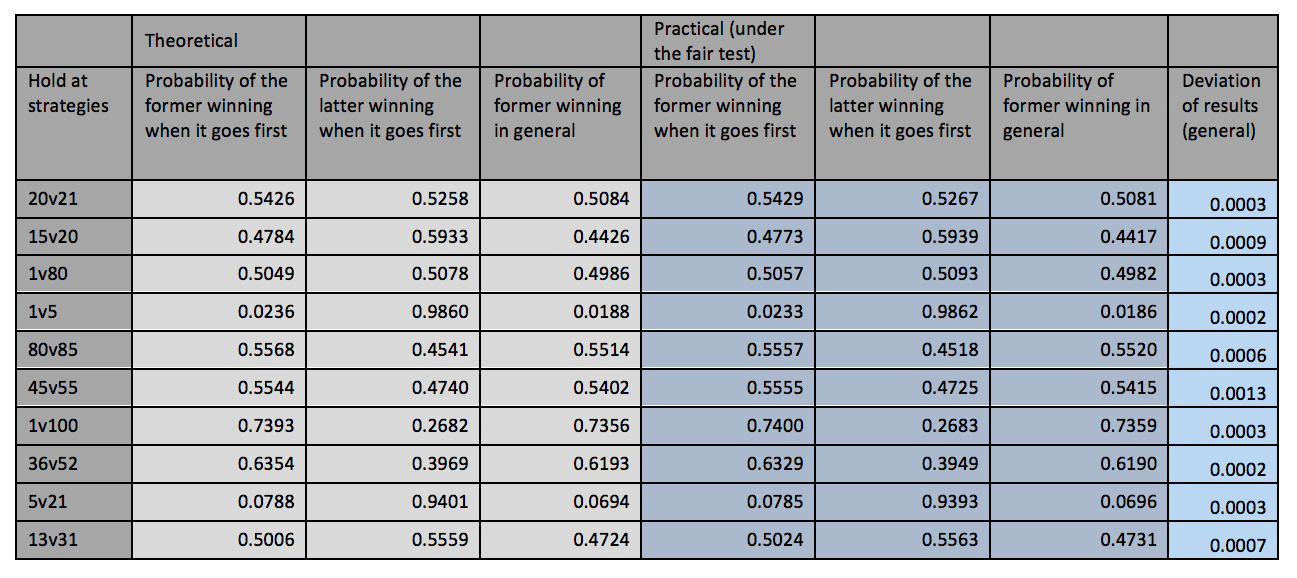
\includegraphics[width=\textwidth]{stats_table}
\caption{stats\label{figure17}}
\end{figure}
Figure \ref{figure17} shows the result from $10$ different games of $2$ different strategies under the fair test. The last column shows the deviation from the theoretical values of the probability and the practical values obtained from the test. By our conditions, if the deviation is greater than $0.025$ then this would imply that the practical results aren’t consistent with the theoretical results implying that the test wasn’t reliable. As you can see the results are all less, and comfortably so, than $0.025$, therefore we can say that the test conducted gives reliable results and is therefore fair.
\subsubsection{Determining whether a strategy is better than another}
There are two ways which we could analyse the results. As we are playing $3000$ games of pig and giving each strategy a score of $1$ for each game they win, we could analyse the score for both strategies and use that to determine whether it is better or worse than the other strategy. Though we are playing $100$ independent $3000$ games and then taking the average score of both strategies, the following method will still apply.\\ \\From looking at our maximal value for the probability in the confidence interval, as $X=np$ where $n=3000$ and $p=0.525$, we can say that if one strategy wins on average $X=3000\times0.525=1575$ then it is better than the other strategy.\\ \\We could also look at the respective probability of the strategies from the theoretical results.  As $p=\dfrac{X}{n}$, if the value for $p$ is outside our determined confidence interval, we can then deduce that one of the strategies is better than the other.
\subsubsection{Statistical findings on the optimal}
It happens to be that simply hold at strategies, i.e. If your turn score is less than $20$ (say, then you always roll, are quite affective (as said by neller?). This made us think that testing our version of the optimal strategy against simply hold at strategies would be a good place to start. We could find the optimal and then play it against numerous hold at strategies and see the results, though we thought it would be good to find whether there was a best hold at strategy so that we only need to use that to analyse our version of the optimal.\\ \\As we saw earlier, Figure \ref{figure17} shows some of the probabilities we obtained from running these tests along with their theoretical probabilities. We decided to run a test, in compliance with our rules for a fair test, in Matlab of every hold at strategy from hold at $1$ to hold at $100$ in order to determine which particular hold at strategy was better than all of the others. As we saw earlier, the strategy hold at $0$ cannot win any games it plays and so, to reduce computing time, we will not include this in our simulations. We wanted to know whether there was one hold at strategy which beat all other strategies, as opposed to finding which one won the most against the others. By this we mean whether the strategies are transitive. By saying that the strategies are transitive, we mean that if we have strategies A, B and C, where A is better than B and B is better than C, then A is better than C also. This would mean that if we find one strategy that is the best, it will beat all other strategies. We ran a Matlab simulation, again alongside our rules for a fair test, which returned a result that confirmed that these simple hold at strategies are in fact transitive.\\ \\After we had looked at the transitivity of strategies, we looked at playing a tournament between all of the ‘hold at’ strategies from $1$ to $100$ in order to find which such strategy was the most superior and beat all of the rest. We again ran this in compliance with our rules for a fair test and the outcome of this tournament was that hold at $25$ came out to be victorious from $10$ tournaments.
\subsubsection{Interesting note}
After we evaluated all of the simple hold at strategies, we decided to look at more complicated strategies that have other rules other than just at what turn score to bank at. When evaluating strategies of this description, we were able to find three strategies that are non-transitive. The strategies we have found that have such properties are named turtle, roll to win and roll and wait. Turtle is a slow strategy, as suggested by its given name, banking on a low score each turn and thus slowly making its way towards $100$. Roll to win is a very simple strategy, where it only banks once the turn score reaches $100$. Roll and wait is a strategy that behaves such that it gets up to a banked score of $80$, before not rolling and waiting for the opponent to catch up, before then rolling to try to win. We ran fair tests between these strategies and have found both practical and theoretical probabilities of each strategy winning against another. When turtle played against roll to win, we got a practical probability that turtle will win with probability of $0.8127$ when going first, compared to $0.1949$ for that of roll to win. Comparatively, we get theoretical probabilities of $0.812840$ for turtle to win going first and $0.195448$ for roll to win. Using these number to calculate who wins in general from multiple games is fairly simple and will be explained further on, but the calculate to be $0.8089$ for turtle winning and $0.1911$ for roll to win to win. This is again showing that our tests are accurate, with very little deviation between the practical and theoretical values. This shows that turtle is a better strategy as both the practical and theoretical probabilities of it beating roll to win lie above $0.525$, the upper bound of our previously stated confidence interval. Similarly, roll to win’s probability lies below the lower bound of $0.475$, further confirming our conclusion that turtle is superior. We then played roll to win against roll and wait and got both practical and theoretical probabilities of $1$ for roll to win winning, regardless of who went first. Roll and wait produces a practical probability of beating turtle $0.7101$ when going first and $0.7062$, whereas the latter wins with probability $0.2983$ when it goes first. This compares to the practical probabilities of $0.710606$ for roll and wait and $0.297148$ for turtle. The probabilities for roll and wait to win clearly lie above the upper bound of our confidence interval, and turtle below the lower bound, hence we conclude that it is the better strategy. As this experiment shows, for both practical and theoretical probabilities, turtle is better than roll to win, roll to win is better than roll and wait, however, roll and wait is better than turtle, giving us a 3-way loop, and hence proving that these such strategies are non-transitive.\\ \\Our function in matlab calculates the probability of a strategy winning given that it starts the game, therefore, theoretically we calculate the general probability of it beating every other ‘hold at’ strategy as follows:\\Let $x$ denote the probability hold at $25$ winning when going first.\\Let $y$ denote that of its opposing strategy when it goes first.\\Let $X$ be the general probability of hold at $25$ winning.\\For $3000$ games, hold at $25$ goes first $1500$ times and second the same amount of times, so we have
\begin{align}
X &= \dfrac{1500(x)+1500(1-y)}{3000}\notag\\
X &= \dfrac{x+(1-y)}{2}\notag
\end{align}
As an example, let’s compare it against hold at $30$. We calculated the probability of hold at $25$ winning when going first as $0.573741$ and that of hold at $30$ as $0.48091$. If we put this in our formula, we get\\ $X=\dfrac{0.573741+(1-0.48091)}{2}=0.546416$. Applying this against all other ‘hold at’ strategies, we can produce the graph in figure \ref{figure17}.
\begin{figure}
\centering
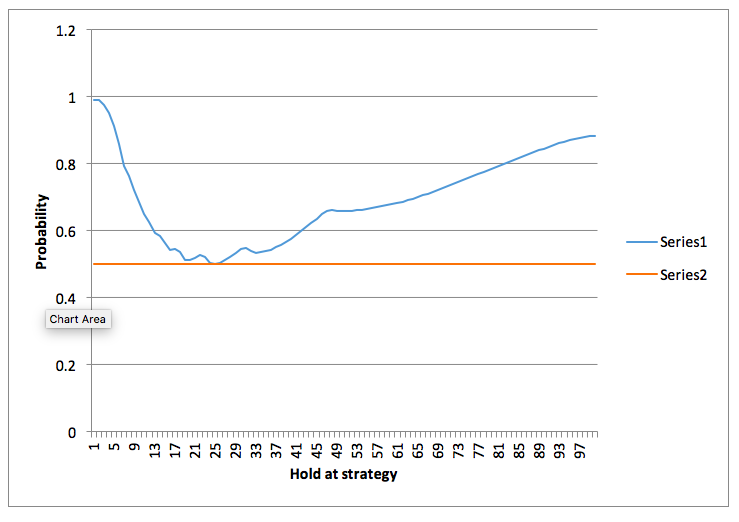
\includegraphics[width=\textwidth]{stats_3}
\caption{\label{figure18}}
\end{figure}
As we can see in figure \ref{figure18}, all of the general probabilities for hold at $25$ winning lie strictly above the line of $y=0.5$, other than when it plays against itself, when it gives a value of $0.5$ as expected. From this, we can deduce that, theoretically, this is also the best of these simple ‘hold at’ strategies.\\ \\Upon finding our ``optimal strategy'', we then had to test it against other strategies in order to show that it is in fact the superior of the two in question and, in turn, the best to play against any given strategy. As we saw from the tournament of all of the ‘hold at’ strategies, and the subsequent table of probabilities, hold at $25$ was the best of the simple old at strategies. As the ‘hold at’ strategies are also transitive, it made sense to test our optimal against this one and then conclude that our strategy beats all of the rest also. We ran the two against each other in line with our fair test and the simulation returned a practical probability of $0.55076$ that our optimal would win when going first and $0.52136$ in general, compared to hold at $25$ winning with probability $0.50804$ when going first and just $0.47864$ in general. As we can see our optimal strategy beats hold at $25$ when going first with a probability that lies above our confidence interval, showing that our strategy is superior. This is also in agreement of theoretical calculations, with our optimal theoretically winning $0.55127$ in general and bank at $25$ winning with probability $0.50914$. As we know that the ‘hold at’ strategies are transitive, this then means that our optimal strategy beats all such simple strategies also.\\ \\We then tested our optimal strategy against that of Neller’s. These simulations returned results of a probability of $0.53182$ when our strategy went first and $0.53176$ when Neller’s went first, which are values within each-others confidence interval which suggest that practically the two strategies could have the same probability. This was also backed up, with theoretical results showing that both neller’s and our optimal won when going first with a probability of $0.53059$. This then gave us a general probability of each strategy winning of $0.5$, showing that our optimal strategy has in fact converged to that found by Neller previously.

\section{Conclusions}
\subsection{Overall findings}
\subsection{Humans playing pig and their interactions}
\textbf{Do players stick to their stated risk preferences?}\\No, we found out that players don’t actually play in align with their stated preferences. It seems that on average, once participants play Pig they have different risk preference. We found that a lot more people are risk seeking than they originally stated. As we can see with the risk preference graphs, we expected the graphs to look like the graphs as shown in the introduction (figure \ref{figure4}). However we found that this wasn’t the case. We explained this as risk preferences are evened out in the long run.\\ \\ \textbf{Player interactions}\\We have concluded that an individual’s strategy is definitely influenced by their opponents. Game 11 (figure \ref{figure13}) and game 14 (figure \ref{figure14}) best represent our overall results found. In summary, we found that players change their strategy and do not stick to the risk preference stated and players copy their opponents strategy. If people stick to mirroring each other they actually have more of a fair chance of winning, whereas if they change their strategies later on in the game it causes a worst outcome. \\ \\ \textbf{Limitations}\\ Our sample size was fairly small. Therefore, if this experiment was to repeated, we would want to ensure that we collected data from a greater number of participants so that we could be more confident in our conclusions.

\subsection{Statsical analysis}
To conclude statistical analysis, we first had to acknowledge that probabilities for our strategies winning could be measured both practically and theoretically and these can often differ greatly. In order to ensure that these were as close as they could be, we needed to create some rules for a fair test by which we would have to follow when playing two strategies against each other, in order to accurately compare them.\\ \\We first noted that a particular strategy will win against itself with a general probability of $0.5$. We then constructed a confidence interval at the $95\%$ significance level with the idea that we didn’t want $p$ to differ more than $0.025$ away from $0.5$, where $p$ denotes the probability of a strategy winning against itself. From this, we could work backwards from our confidence interval and find the optimal number of games, $n$, required for one single fair test. This method produced $n=1537$. However, we saw from figure \ref{figure15} that this value of $n$ gave too many outliers in the data, so we instead chose $3000$ as it appeared accurate for our particular confidence interval. As this number still produced some outlying data, we decided to run $100$ fair tests in order to minimise the error as much as we could in order to obtain accurate practical probabilities against theoretical ones. \\ \\We decided first to look at simple ‘hold at’ strategies and found them to be transitive. By this, we mean, for three strategies A, B and C, if A is better than B and B is better than C, then A is better than C. This means we could have one strategy superior than the rest and we found this to be hold at 25, when we ran a tournament between the strategies.\\ \\We were then required to test if the optimal strategy that we thought we had found was in fact superior. As we knew the ‘hold at’ strategies to be transitive, we only needed to test it against the best of these in order to know that it was better than the rest, assuming that it won. Our optimal strategy won with general probability of $0.52136$, thus allowing us to conclude that it was better than all of the ‘hold at’ strategies.\\ \\We then tested our optimal against that found by Neller\citep{neller2004optimal} to see if our strategy had in fact converged to this. Both strategies, when going first, won with the same probability of $0.53182$, giving a general probability of $0.5$ for each strategy. We could then conclude that our strategy was in fact the same as the optimal that Neller had found and written about himself.

\nocite{*}
\bibliographystyle{plain}
\bibliography{Pig_bib}
\end{document}
